% preamble %
\documentclass[12pt]{article}
\usepackage{amsfonts}
\usepackage{fancyhdr}
\usepackage{comment}
\usepackage[a4paper, top=1cm, bottom=1.5cm, left=2cm, right=2cm]{geometry}
\usepackage{enumitem}
\usepackage{times}
\usepackage{changepage}
\usepackage{amssymb}
\usepackage{graphicx}
\usepackage{tabularx}
\usepackage{titlesec}
\usepackage{hyperref}
\usepackage{changepage}
\usepackage[parfill]{parskip}
\usepackage{wrapfig}
\usepackage[export]{adjustbox}
\usepackage{multirow}
\usepackage{array}
\usepackage[table]{xcolor}
\usepackage{longtable,booktabs}

% settings %
\setcounter{secnumdepth}{2} % enumerate
\setcounter{tocdepth}{2}    % TOC entries
\renewcommand{\contentsname}{Innholdsfortegnelse}
\newcounter{fkcounter}
\newcounter{fksubcounter}[fkcounter]
\newcounter{ifkcounter}
\newcounter{ifksubcounter}[ifkcounter]
\titlespacing*{\paragraph}{\parindent}{1ex}{1em}

% commands %
    % counters %
\newcommand*{\FK}{\stepcounter{fkcounter}\textbf{ID: FK\arabic{fkcounter}\\}}
\newcommand*{\FKsub}{\stepcounter{fksubcounter}\textbf{ID: FK\arabic{fkcounter}.\arabic{fksubcounter} \quad}}
\newcommand*{\IFK}{\stepcounter{ifkcounter}\textbf{ID: IFK\arabic{ifkcounter}\\}}
\newcommand*{\IFKsub}{\stepcounter{ifksubcounter}\textbf{ID: FK\arabic{ifkcounter}.\arabic{ifksubcounter} \quad}}
\newcommand{\invis}{\phantom{a}}

    % colors %
\newcommand{\cellr}{\cellcolor{red!25}}
\newcommand{\cello}{\cellcolor{orange!25}}
\newcommand{\celly}{\cellcolor{yellow!25}}
\newcommand{\celll}{\cellcolor{lime!25}}
\newcommand{\cellg}{\cellcolor{green!25}}

% environments %
\newenvironment{subreq}{\begin{adjustwidth}{1cm}{}}{\end{adjustwidth}}

% document %
\begin{document}
\title{%
    Kravspesifikasjon\\
    \large Reservasjonssystem for parkeringsplasser}
\author{%
    Gruppe 12:\\
    Jonas Eliassen\\
    Mats Engelien\\
    Lars Erik Faber\\
    Håkon Marthinsen\\
    Charis Schille}
\date{}
\maketitle

\newpage

\tableofcontents

\newpage

\section{Problemstilling}

Ofte finner man ikke parkeringsplass mens man er i farta. Det er tett på senterene, gateparkering er privat eller ulovlig og man har ofte dårlig tid. Gjerne etter litt leting finner man en parkering 500 meter unna, og når man kommer dit er det selvfølgelig fullt. Hvordan kan man unngå å miste så mye tid, og i tillegg finne en parkeringsplass?

\section{Løsningen}
Tjenesten baserer seg på delingsøkonomi og enheten som deles er parkeringsplasser. Ideen er at bedrifter og enkeltpersoner kan registrere en eller flere parkeringsplasser de eier for utleie til enkeltpersoner. Dermed kan disse utleierene tjene penger passivt, samt gjøre det enklere for privatpersoner å forsørge parkering. Parkeringsplassen de legger ut vil være merket med bredde, lengde og høyde, samt om den er reservert for el-biler eller handicappede. På denne måten kan alle som bruker tjenesten få et godt innblikk i parkerings-bildet.

Bruker logger inn som en bedrift eller en vanlig bruker. Brukere kan redigere og legge ut sine registrerte parkeringsplasser, samt leie parkeringsplasser fra andre brukere. Bedrifter kan kun legge ut parkeringsplasser, men har muligheten til å legge til brukere som medlemmer av bedriften. Dette gir de spesialtillatelse til parkeringsplasser som er reservert kun for medlemmer av en spesifikk bedrift. Medlemmer av bedriften vil også kunne legge ut og merke parkeringsplasser for andre bedrifter.

Tjenesten er bygget opp slik at alle brukere har tilgang til en feed som viser en opplisting av de mest relevante parkeringsplassene, en side for registrering av parkeringsplasser og en profilside. For å kunne reservere en parkeringsplass, må bruker oppgi informasjon om bilen de benytter. På feeden rangeres de tilgjengelige parkeringsplassene etter avstand til bruker eller et spesifikt område som bruker spesifiserer, og vises kun dersom de er passende med bilen. Bruker kan også trykke seg inn på et spesifikt innlegg for å se mer detaljer om parkeringsplassen som leies ut, og kan legge en anmeldelse på parkeringsplasser de har brukt. På denne måten får utleiere tilbakemelding på hva de gjør riktig og hva de gjør galt, som bidrar til å øke engasjementet til å gjøre en god jobb.

Kunde av tjenesten vil kunne opprette administratorbrukere som har spesielle egenskaper for administrering av feeden og brukerene. Dette vil være nødvendig for å minke upassende/ulovelig innhold og øke brukeropplevelsen.

\section{Begrensninger og antagelser}

    \subsection{Begrensninger}
        \textbf{Tilkobling til en tredjepart :} Dette er for at brukerene av applikasjonen skal kunne betale for tjenesten og for de som gir den tjenesten skal kunne få betalt for det.
        
        \textbf{Servere rundt i landet :} Fordelene med å ha flere servere rundt i landet er for å gi en bedre flytt i på systemet for brukerene av applikasjonen.
        
        \textbf{Cookies :} Dette blir brukt for å få tilgang til enkelte funksjoner i applikasjonen og gjøre det så enkelt og trykt for en bruker av applikasjonen.
        
        \textbf{Googlemaps API :} Fordelene med å bruke Googlemaps er grunnet oppdattering og ytelse, men å bruke cookies så blir det enkelt for en bruker å finne fram til en parkeringsplass etter hvor de er.
        
        \textbf{Data lagring :}

    \subsection{Antagelser}
        \textbf{Opprette en parkeringsplassen i applikasjonen :} Når en bruker skal opprette en parkeringsplass for første eller for de neste alle andre gangene fremover, så skal det det være så enkelt og kjapt som mulig at de ikke får følesen av at de kaster bort tid (og penger). Det skal være så enkelt at når en bruker har logget seg inn så skal det stå opprett en parkeringsplass. Der skal de kunne fylle in informasjon om, hvor mange etasjer det er, hvor stort er område er det, hvor ligger den, skal den ha noen parkeringsregler for område. Når eieren for parkeringsplassen har opprette starts delen for parkeringsplassområdet så er det vikitg at de kan fylle innholdet på parkeringsplassen, som hvor mange parkeringsplasser det i hver etasjer, hva slags parkeringsplass er det (er plassen handicappede, eletrisk, motorsykkel osv.), skal parkeringsplassen ha en bestemt ID og time prisen for å parker hos dem. Imens eieren for parkeringsplassen oppretter den så er det vikitg at systemt lagrer / tar backups av det de gjør i tilfelle noe skulle skje. Når de er ferdig med å opprette en parkeringsplass, så skal det være så enkelt at de kan si at den er åpen for bruk og alt etter dette her skal skje automatisk, når det gjelder å leie fra dem.
        
        \textbf{Oppdater en parkeringsplassen i applikasjonen :} Eieren av en parkeringsplass vil kanskje endre på noe i den fysiske eller det som ligger ut i applikasjonen om det skulle være, om det er å legge til en ekstra etasje, flere/fære parkeringsplasser, endring av strukturen av parkeringsplassen, informasjonsfeil. Da er det vikitg at de kan endre på ting med på trykk. De skal finne en knapp vedsiden av parkeringsplassen som de eier på applikasjonen i minne parkeringsplassener. Når de trykker på rediger parkeringsplass, så skal de få muligheten til å rediger/endre på informasjonen som er lagret i den parkeringsplassen. Når eiren er ferdig med å rediger/endre så skal de kunne trykke lagre og da vil systemet gjøre resten.
        
        \textbf{Leie :} Når en bruker trenger et sted å parkere, så skal det være så enkelt som å logge seg på og finne knappen lei en parkeringsplass. Når brukeren har trykket på lei en parkeringsplass så vil de bli ført til en side der de kan søke etter bestemte parkeringsplasser etter dems behov, om det er handicappede parkering, eletrisk parkering eller om det er en normal parkeringplass. De har også muligheten for å bestemme hvor de skal parker om det er på dems vanlige parkeringsplass eller om det er på et nytt område. Når de har valgt hvor de skal parker og oppfylt alt av informasjon som trengs så skal de kunne betale for det, men før de kan betale for parkingen så må de velge tiden fra og til -tiden de skal stå der. Da vil applikasjoen kalkulere prisen for tiden bruken skal stå der (time pris) og de skal de kunne betale for det. Etter de har trykket betal så skal de få en melding om at det er godkjent og en kvitering for at de har betalt for den.
        
        \textbf{Administrator og administrer :} Det er viktig som en administrator at alt som i applikasjoen som vises fra til de andre brukeren på stemmer. At ingeng lager flaske brukere og oppretter falske parkeringsplasser som kan bli brukt til svindel eller stjeling av andres privatinformasjon. Det kan hende at man må slette disse brukerne eller banlyse dem og det samme gjelder for de falske parkeringsplassen. 


\section{Ansvarsområde og Avhengigheter}
Tjenesten skal dekke områder som framvisning, utleie og reservasjon av parkeringsplasser, brukerinnstillinger, lagring av brukerdata gjennom cookies, lagring av parkeringsplasser, lagring av brukeranmeldelser. Tjenesten skal ikke håndtere transaksjoner, men etterspør bank. GPS koordinater håndteres av en tredjepart. Tjenesten har heller ikke ansvar for hosting.

Applikasjonen bygger på automatiseringsverktøy Maven med JDK versjon 11. Jackson brukes for datalagring for datalagring og Vue som er et åpent visningsrammeverk og brukes for visning av tjenesten. Javalin er web-rammeverket som brukes, og testene kjøres med JUnit.

Her er en fullstendig liste:\\
\textbf{JavaJDK v11} For kjøring av kode.
\\\textbf{fasterxml.jackson 2.9.9} Lagring av data.
\\\textbf{maven 3.8.0} Bygge automatiseringsverktøy.
\\\textbf{webjars vue 2.6.10} For det visuelle nettsidene.
\\\textbf{javalin 3.11.0} Rammeverk for nettsiden.
\\\textbf{JUnit 5.7.0} For å testeing av kodeoppsett.
Nets 


\section{Funksjoner i applikasjonen}

Programmet henter inn info om brukere, poster, parkeringsplasser og reservasjoner fra en database(i dette tilfellet json-filer). Det programmet gjør nå er å hente inn data fra controller til javalin som generer front-end for oss. Hver side henter da ut nødvendig info hva hver .json fil slik at nødvendig informasjon som adresse og ledighet til leie vises.

Bruker -  Det er mulig å vise oversikt over parkeringsplasser, trykke seg inn til en parkeringsplass, og å legge til en reservasjon, brukeren kan også se oversikt over p-plassene som den har reservert. Det er mulig å legge ut en ny parkeringsplass som en utleier. Det er mulig å vise bilder av parkeringsplassen via et link system, da opplastning direkte til siden ikke er lagt inn. 

Corporation bruker - kan kun legge ut parkeringsplasser. Dette gjør man ved å gå til “My parking spots” hvor “Create new parkingspot” står øverst. For å lage et nytt parkingeringsobjekt må man trykke på denne knappen og fylle ut all nødvendig info(feilmelding dersom ikke alt har noen verdi), og man kan i tillegg velge ved bruk av ikoner dersom det er handikappet eller el-bil plass. Corporation skal kunne få betalt for å leie ut p-plasser.

Admin - Denne brukeren kan suspendere eller slette/banlyse brukere, slette poster og parkeringsplasser. Dette er en bruker-type som i senere iterasjoner kan gi rettigheter til andre brukere (f.eks. modererings-brukere).


\section{Begreper og definisjoner}

\begin{center}
    \begin{tabular}{|p{4cm}|p{12cm}|} 
        \hline
        \bf Begrep & \bf Beskrivelse\\
        \hline
        Applikasjon &  Et programvare som benytter datamaskinens ressurser til en oppgave som brukeren ønsker utført\\
        \hline
        Cookies & En type fil som brukes midlertidig for å lagre informasjon\\
        \hline
        Bruker & Besøkende som samhandler med systemet\\
        \hline
        Brukerkonto & En som kan kun leie parkeringsplasser\\
        \hline
        Bedriftskonto & En som kan kun leie ut parkeringsplasser til andre\\
        \hline
        Administrator & Brukerkonto med administratorrettigheter\\
        \hline
        Feed & Opplisting av innlegg\\
        \hline
        Tjenesten & Tjenesten denne dokumentasjonen omhandler\\
        \hline
        Systemet & Det underliggende systemet til tjenesten\\
        \hline
        Personas & Er et annet ord for rollefigur, enkeltmenneske, karakterpersonlighet\\
        \hline
        ID & Identifikator\\
        \hline
        FK & Funksjonelt Krav (brukes som ID)\\
        \hline
        IFK & Ikke-Funksjonelt Krav (brukes som ID)\\
        \hline
        Innlegg & Brukerinnlegg i systemet (post) som består av en eller flere parkeringsplasser\\
        \hline
        Produktet/ Tjenesten & Applikasjonen som dokumenteres\\
        \hline
        Kunde & Gruppe som eier produktet\\
        \hline
        Push-notifikasjoner & Varsler på desktop eller mobil \\
        \hline
        Cookies & Informasjonskapsler \\
        \hline
        TOS & Terms of Service, liste over bruksrettigheter og bruksområde for brukerdata \\
        \hline
    \end{tabular}
\end{center}

\section{Brukerklasser}
En oversikt over roller og egenskaper for de forskjellige brukerklassene.

    \subsection{Bruker}
    Brukerkontoen er en standardkonto som hvem som helst kan opprette. Som en bruker, kan man registrere sine egne parkeringsplasser og leie andre brukeres parkeringsplasser i perioder. Alle brukere har sin egen profilside der de kan redigere generell informasjon og innstillinger. Brukere kan gi anmeldesler/tilbakemelding på hverandre sine innlegg, og vil bli varslet dersom en annen bruker skriver en anmeldelse på sin parkeringsplass. Ved registrering av parkeringsplass, bestemmer man selv pris og tiden den er tilgjengelig, og den vil automatisk bli vist for andre brukere via feeden eller profil. Man må først registrere bilen man parkerer med før man kan reservere en parkeringsplass.

    \subsection{Bedrift}
    Det er kun organisasjoner som har tilgang til å opprette en bedriftskonto, da de må ha et organisasjonsnummer. Bedriftskontoen er sammensatt av flere brukerkontoer. En brukerkonto som er medlem av en bedrift har spesialtilgang til parkeringsplasser markert for generelle eller spesifikke bedrifter. Bedriftskontoen kan legge ut parkeringsplasser, men kan ikke leie en parkeringsplass. Det er kun bedrifter som kan markere parkeringsplasser for andre bedrifter.

    \subsection{Administrator}
    En administrator ligner en vanligbrukerkonto, men har moen ekstra rettigheter for administraring. De har full makt til å slette brukere, bedrifter, innlegg, parkeringsplasser, og anmeldelser, samt suspendere og oppheve brukerkontoer. Administrator er essensiell for å vedlikeholde en god brukeropplevelse og rettferdiggjøre systemet for alle brukere.

\section{Personaer}

    \subsection{Jørgen Moe}
    
\includegraphics[scale=1]{bilder/personaer/persona_jorgen.jpg}\\
    \textbf{Alder:} 34\\
    \textbf{Jobb/Rolle:}
    Økonom\\
    \textbf{Beskrivelse:}\\
    Jobber som økonom. Han skal grave i gården og lage ny parkeringsplass. Han vet ikke hvor lang tid det kommer til å ta, og han kommer ikke til å ha et sted å parkere i mellomtiden.\\
    \textbf{Motivasjon:}\\
    Han har ikke parkeringsplass hjemme, så han trenger en parkeringsplass i nærheten.\\
    \textbf{Behov:}\\
    Han må kunne forlenge antall dager han låner en parkeringsplass\\
    \textbf{Tekniske ferdigheter:} Gode
    

    \subsection{Siggurd Olson}
    
\includegraphics[scale=1]{bilder/personaer/persona_siggurd.jpg}\\
    \textbf{Alder:} 42\\
    \textbf{Jobb/Rolle:} Ledelse i bedrift\\
    \textbf{Beskrivelse:}\\
    Jobber i ledelsen i en bedrift. Det er ikke alltid han får en plass til å parkere i byen når han skal på jobb.\\
    \textbf{Motivasjon:}\\
    Parkeringsplassene i byen er fullstappa.\\
    \textbf{Behov:}\\
    Han må kunne parkere nærmere arbeidsplassen og sikre seg parkeringsplass ved et møte.\\
    \textbf{Tekniske ferdigheter:} Gode

    \subsection{Karina Gausrud}
    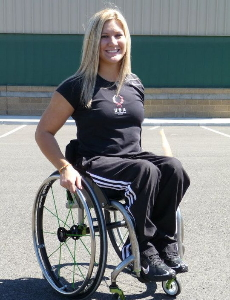
\includegraphics[scale=1]{bilder/personaer/persona_karina.jpg}\\
    \textbf{Alder:} 22\\
    \textbf{Jobb/Rolle:} Uføre\\
    \textbf{Beskrivelse:}\\
    Karina er en rullestolbruker som trenger handicap-parkering. Hun vil helst parkere så nærme målet sitt som mulig, men vet ikke om det finnes en ledig handicap-parkeringsplass. Hun vil heller ikke risikere at stedet ikke tilbyr parkeringsplass for handicappede.\\
    \textbf{Motivasjon:}\\
    Hun trenger en oversikt over ledige handicap-parkeringsplasser.\\
    \textbf{Behov:}\\
    Hun må være sikker på at hun får en handicap-parkeringsplass\\
    \textbf{Tekniske ferdigheter:} Gode

    \subsection{Karin}
    
\includegraphics[scale=1]{bilder/personaer/persona_karin.jpg}\\
    \textbf{Alder:} 34 \\
    \textbf{Jobb/Rolle:} Selger\\
    \textbf{Beskrivelse:}\\
    Karin er dør-til-dør selger, hun kjører til nabolagene hun jobber i hver dag, men det er vanskelig å finne parkering, som gjør at hun taper tid og penger mens hun leter. Derfor åpner hun appen og booker parkeringsplasser for områdene hun skal jobbe den neste måneden. Nå føler Karin at hun har en mindre ting å tenke på.\\
    \textbf{Motivasjon:}\\
    Han har ikke parkeringsplass hjemme, så han trenger en parkeringsplass i nærheten\\
    \textbf{Mål:}\\
    Karin ønsker å eliminere en del av hverdagen som er unødvendig og som koster henne tid og penger. Karin forventer at hun skal finne parkering, og kunne booke det for måneden fremover, eller på dagen om nødvendig.\\
    \textbf{Reisen:}\\
    For å oppnå dette er Karin nødt til å finne utleiere som ønsker kort-tid/dagsutleie, så hun er nødt til å søke området hun skal til, og filtrere til dette alternativet. Deretter kan hun velge sted å parkere basert på beliggenhet og pris i forhold til området hun utvalgte seg.\\
    \textbf{Følelser:}\\
    Karin føler seg frustrert når hun kjører rundt nabolaget hun skal banke dører i, men aldri klarer å finne et sted det er lov å parkere. Karin er på sitt lykkeligste når hun åpner appen for å sjekke hvor hun har bestilt parkering, og vet at hun ikke trenger å tenke på å lete igje\\
    \textbf{Tekniske ferdigheter:} Gode

    \subsection{Jørn Berg}
    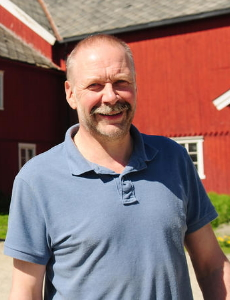
\includegraphics[scale=1]{bilder/personaer/persona_jorn.jpg}\\
    \textbf{Alder:} 56\\
    \textbf{Jobb/Rolle:} Bonde\\
    \textbf{Beskrivelse:}\\
    Jørn bor i nærheten av et vakkert tjern som er populært blant unge å bade i, men siden det ikke er noen parkeringsplass der må folk parkere langs veien. Jørn eier en fin tomt i nærheten der folk kan parkere tryggere.\\
    \textbf{Motivasjon:}\\
    Han vil at tilby parkeringsplasser slik at ungdommene mer sannsynligvis kommer tilbake til tjernet og bader.\\
    \textbf{Behov:}\\
    En omtale system som kan bidra å spre det gode rykte videre. Han vil leie ut tomten for en inntekt ved siden av gårsdriften.\\
    \textbf{Tekniske ferdigheter:} Dårlig

\section{Funksjonelle krav}

    \subsection{Kontoopprettelse}
        
        \subsubsection{Bruker skal kunne opprette en brukerkonto}
        \FK
        For å oppgrette en brukerkonto, må bruker oppgi brukernavn, passord, e-post og telefonnummer.

            \begin{subreq}
                \FKsub Brukernavn og passord må være unike.
            \end{subreq}

        \subsubsection{Bedrifter skal kunne opprette en bedriftskonto}
        \FK
        For å opprette en bedriftskonto, må bedriften må oppgi brukernavn, passord, e-post, bedriftsnavn og organisasjonsnummer.

            \begin{subreq}
                \FKsub Brukernavn, passord, bedriftsnavn og organisasjonsnummer må være unike.
            \end{subreq}

        \subsubsection{Kunden skal kunne opprette brukerkonto med administratorrettigheter}
        \FK
        Bare kunde av applikasjonen kan opprette denne brukerkontoen. For å opprette denne kontoen må kunden oppgi et brukernavn, passord og telefonnummer.

            \begin{subreq}
                \FKsub Brukernavn, passord og telefonnummer må være unike.
            \end{subreq}

        \subsubsection{Systemet skal verifisere registreringen}
        \FK
        Systemet må verifisere registreringen via verifiseringskode som sjekkes. Denne må bli sendt til brukeren slik at de kan skrive inn koden til programmet. Hvis koden stemmer med den som er lagret i databasen, er registreringen verifisert. Hvis ikke skal de få en feilmelding på samme siden. Etter verifisering lagres brukerdataen i databasen.

        \subsubsection{Dirigere opprettet bruker}
        \FK
        Etter opprettelse av konto skal bruker automatisk bli ført til startsiden.
    
    \subsection{Innlogging}

        \subsubsection{Bruker skal kunne logge inn som en brukerkonto eller bedriftskonto}
        \FK
        Bruker skal kunne velge å logge inn som en brukerkonto eller bedriftskonto, og så fylle ut tekst-felter med de samme opplysningene som da de opprettet kontoen sin.

        \subsubsection{Systemet skal verifisere innloggingen}
        \FK
        Dersom innloggingsopplysningene er korrekte i forhold til opplysningene i brukeropprettingen, skal brukeren bli logget inn. Dersom de er ukorrekte, skal brukeren få en feilmeldingen på hva som gikk galt.

        \subsubsection{Dirigere innlogget bruker}
        \FK
        Etter vellykket innlogging skal bruker bli ført til startsiden.

        \subsubsection{Bruker skal kunne tilbakesette passord}
        Brukere har valg om å tilbakesette passord hvis de har glemt dette. I så fall skal bruker bli sendt verifiseringskode som skrives inn i et nytt felt for å verifisere at det er samme bruker. Hvis koden stemmer kan bruker skrive inn nytt passord som skal brukes fremover.

    \subsection{Verifiseringskode}

        \subsubsection{Systemet skal verifisere bruker gjennom en kode}
        \FK
        Denne koden blir brukt til blant annet Kontoopprettelse, passordbytte og to-faktor autentisering. Hensikten er å gjenkjenne brukeren som gjør sikkerhetskritiske handlinger på sin profil. Når bruker gjør en av disse handlingene blir koden midlertidig lagret i databasen, og videre sendt til bruker. Bruker må skrive koden inn i et tekst-felt, der den blir sjekket opp med den opprinnlige koden lagret i databasen. Hvis den stemmer er brukeren verifisert.

            \begin{subreq}
                \FKsub Koden skal være fire-sifret

                \FKsub Koden skal bli sendt via sms
            \end{subreq}

    \subsection{Presentasjon av parkeringsplasser (Feed)}

        \subsubsection{Feeden skal oppliste relevante parkeringsplasser}
        \FK
        Alle brukertyper skal ha tilgang til en opplistingen som består av innlegg fra andre brukere. Det er her brukere ettersøker og reserverer parkeringsplasser. Standaropplistingen rangeres etter nærmest avstand fra posisjonen til brukeren.

            \begin{subreq}
                \FKsub Posisjonen hentes via cookies.
            \end{subreq}
        
        \subsubsection{Bruker skal kunne sette et filter på feeden}
        \FK
        Opplistingen rangeres via et brukervalgt filter. Filteret bestemmer om opplastingen rangeres basert på nærmest avstand, lavest til høyest pris, høyest til lavest pris, parkeringsplasstype og om den leies ut av en brukerkonto eller bedriftskonto.

        \subsubsection{Bruker skal kunne søke etter en lokasjon}
        \FK
        Feeden skal rangere parkeringsplassene basert på avstand i forhold til denne lokasjonen.

            \begin{subreq}
                \FKsub Søkefeltet skal akseptere adresse.

                \FKsub Søkefeltet skal akseptere koordinater.
            \end{subreq}

    \subsection{Leie parkeringsplass}

        \subsubsection{Bruker skal kunne leie parkeringsplass som en brukerkonto}
        \FK
        Som en brukerkonto skal bruker kunne leie en eller flere parkeringsplasser. Dette gjøres ved at systemet oppretter en reservasjon for der parkeringsplassen knyttes opp til brukeren som leier den.

        \subsubsection{Varsel på utløpstid}
        \FK 
        Når en reservert parkeringsplass holder på å gå tom for tid, så skal brukeren som har leid parkeringsplassen få en varsel om at den holder på å gå ut minst 30 minutter før.

            \begin{subreq}
                \FKsub Varselet skal gå gjennom SMS og push-notifikasjoner
            \end{subreq}

    \subsection{Tilbakemelding på innlegg (Anmeldelser)}

        \subsubsection{Bruker skal kunne gi tilbakemelding på et innlegg}
        \FK
        Dersom brukeren har brukt en parkeringsplass, skal de kunne gi tilbakemelding på innlegget til den parkeringsplassen. Innlegget må minst bestå av en poengsum. Om ønskelig kan bruker også legge til en kommentar. Tilbakemeldingen skal lagres i databasen og tilknyttes innlegget.

            \begin{subreq}
                \FKsub Hver bruker kan bare skrive en anmeldelse per innlegg.

                \FKsub Kommentaren skal være på maks 130 tegn.

                \FKsub Poengsummen skal være fra 1 til 5, der 5 er den høyeste poengsummen.
            \end{subreq}

        \subsubsection{Tilbakemeldinger skal vises på hvert innlegg}
        \FK
        Alle anmeldelser som tilhører et innlegg skal vises på listeform på innlegget, der den nyeste tilbakemelding ligger øverst.
            
            \begin{subreq}
                \FKsub Hver tilbakemelding skal vise poengsummen, kommentaren og brukernavn til de som lagde den.
            \end{subreq}

        \subsubsection{Utleier skal kunne få tilbakemeldingene via e-post}
        \FK
        Ved valg har utleier mulighet til å få tilsendt alle tilbakemeldinger på e-post.

    \subsection{Opprette parkeringsplasser}

        \subsubsection{Brukerkonto og bedriftskonto skal kunne registrere en eller flere parkeringsplasser}
        \FK
        For å registrere en parkeringsplass må følgende oppgis:
            \begin{itemize}
                \item Bredde, lengde, høyde i centimeter
                \item Antall parkeringsplasser
                \item Type parkeringsplass (om det er handikapparkering, eletriskparkering, osv.)
                \item Etasje
                \item Pris (dette skal kunne endres mauelt eller automastisk i etter kant)
                \item Postaddresse
                \item Gateaddresse
                \item Gatenummer
            \end{itemize}
        Etter opprettelsen lagres parkeringsplassen i databasen.

            \begin{subreq}
                \FKsub Bedriftskonto skal kunne markere en parkeringsplass for en spesifikk bedrift eller for bedrifter generelt

                \FKsub Parkeringsplassen skal knyttes til en unik ID
                
                \FKsub Parkeringsplassen skal knyttes til brukeren som opprettet den.
            \end{subreq}

    \subsection{Leiebetingeleser}

        \subsubsection{Pris per time skal bestemmes av utleier}
        \FK
        Dette er prisen som parkeringsplassen leies ut for (per timer) og bestemmes av bruker som registrerte parkeringsplassen. Den bestemmes på hver individuelle parkeringsplass.

            \begin{subreq}
                \FKsub Prisen skal kunne oppdateres etter opprettelsen.
            \end{subreq}

        \subsubsection{Tiden skal bestemmes av bruker}
        \FK
        Dette er fra-tid og til-tid som parkeringsplassen kan leies av andre brukere.

        \subsubsection{Brukere skal kunne se ut ifra innlegget om parkeringsplassen er ledig eller ikke}
        \FK
        Ledig-statusen regnes ut dersom den tilgjengelige tiden samsvarer med nåværende klokkeslett.

            \begin{subreq}
                \FKsub Hvis en annen bruker låner parkeringsplassen, så skal tiden den er opptatt bli trukket fra det totale tilgjengelige tidsintervallet.
            \end{subreq}

        
        
    \subsection{Betaling}

        \subsubsection{Bruker skal betale utleieren for å opprette en reservasjon}
        \FK
        Bruker betaler for antall timer de ønsker å leie parkeringsplassen.

        \subsubsection{Tredjepart}
        \FK
        Når en bruker sender inn en forespørsel om å kunne leie en parkeringsplass, så må tredjepart verifisere kjøpet før en bruker kan leie.        

    \subsection{Administrering}

        \subsubsection{Administrator skal kunne bannlyse bruker}
        \FK
        Administrator skal ha full rett til å bannlyse en vilkårlig bruker.
        
            \begin{subreq}
                \FKsub Den bannlyste brukeren skal få beskjed om bannlysingen via e-post og direkte i systemet.
            \end{subreq}

        \subsubsection{Administrator skal kunne slette bruker}
        \FK
        Administrator skal ha full rett til å slette individuelle brukere slik at all tilhørende data blir også slettet fra databasen.
        
            \begin{subreq}
                \FKsub Den slettede brukeren skal få beskjed om slettingen via e-post.
            \end{subreq}

        \subsubsection{Administrator skal kunne slette tilbakemeldinger}
        \FK
        Administrator skal ha full rett til å slette individuelle tilbakemeldinger på andre innlegg slik at de fjernes både fra grensesnittet og databasen.

        \subsubsection{Administrator skal kunne slette innlegg}
        \FK
        Administrator skal ha full rett til å slette individuelle innlegg.

            \begin{subreq}
                \FKsub Bruker som lagde innlegget skal få beskjed om slettingen via e-post og direkte i systemet.
            \end{subreq}

        \subsubsection{Administrator skal kunne slette parkeringsplasser}
        \FK
        Administrator skal ha full rett til å slette individuelle parkeringsplasser.

            \begin{subreq}
                \FKsub Bruker som opprettet parkeringsplassen skal få beskjed om slettingen via e-post og direkte i systemet.
            \end{subreq}

        \subsubsection{Administrator skal kunne slette reservasjoner}
        \FK
        Administrator skal ha full rett til å slette individuelle reservasjoner.

            \begin{subreq}
                \FKsub Bruker som opprettet reservasjoner skal få beskjed om slettingen via e-post og direkte i systemet.
            \end{subreq}

        \subsubsection{Bedrift skal ha administrerende rettigheter på deres egne innlegg}
        \FK
        Dette innebærer at bedriften kan blokkere brukere av deres egne parkeringsplasser fra å bruke de igjen og slette tilbakemeldinger på deres egne innlegg.

        \subsubsection{Bruker skal kunne rapportere andre brukere sine innlegg}
        \FK
        Brukere har frihet til å rapportere andre brukere sine innlegg. Rapporteringen skal bestå av en begrunnelse.

            \begin{subreq}
                \FKsub Brukeren som har lagd innlegget skal få varsel via e-post om rapporteringen.
            \end{subreq}

        \subsubsection{Bruker skal kunne rapportere andre brukere}
        \FK
        Brukere har frihet til å rapportere andre brukere. Rapporteringen skal bestå av en begrunnelse.
    
            \begin{subreq}
                \FKsub Brukeren som har lagd innlegget skal få varsel via e-post om rapporteringen.
            \end{subreq}

    \subsection{Persistent data}

        \subsubsection{Systemet skal lagre informasjon om parkeringsplasser}
        \FK
        Systemet skal lagre all informasjon relatert til enhver parkeringsplass i en tabell i en database, slik at endringene gjenstår.

\section{Ikke funksjonelle krav}

    \subsection{Tilgjengelighet}
    \IFK
    All brukere skal ha tilgang til applikasjonen til enhver tid.
    
    \subsubsection{Bruker kvalifikasjon}
    \IFK
    Brukere må minimum være minimum 16 år, og ha gyldig førerbevis.
    
    \subsection{Sikkerhetskopi(Backup)}
    \IFK
    Sikkerhetskopiering av database skal skje hver 24 time kl 04.00

    \subsection{Dependency på tredjepart}
    \IFK
    Betaling verifiseres og håndteres av NETS

    \subsection{Legal and licensing issues}
    \IFK
    Brukeren skal få en Terms of service hvor de får informasjon om hvordan informasjonen deres brukes, og hva de har rettigheter på, og hvilke rettigheter vi har ovenfor deres bruk av tjenesten.


    \subsection{Response time - Lokalt}
    \IFK
    Launch av Javalin til localhost:7000 skal ta mellom 800 - 900 ms.
        \subsubsection{Page loading}
        \IFK
        Lasting av side skal ta ca 1 sekund.


    \subsection{Personvern}
    \IFK
    Lagring av persondata skal skje i henhold med oppdatert GDPR-lovverk.

   
    \subsection{Sikkerhet}
    \IFK
    Programvareutviklingen skal skje i samråd med datatilsynets anbefalning om innebygd personvern.

    \subsection{Supportability}
    \IFK
    Systemet skal være lag-delt slik at det er kost-effektivt å vedlikeholde eller gjøre endringer.

    \subsection{Usability}
    \IFK
    Alle metoder/funksjoner som er ofte i bruk skal ha tester for å sikre at programmets viktigste funksjoner holder.
        
    
    \subsection{Compliance}
    \IFK
    Parkeringsplasser registrert må følge nasjonale, regionale og lokale retningslinjer for manuvreringsrom og areale for parkeringsplass.

% @TODO: Fremtidig implementasjon
%
% \subsubsection{Bruker kan ha flere biler}
% Når en kunde skal resevere en parkeringsplass, så kan det hende at de har tilgang på flere biler og de skal de bilen være lagret etter bruk i brukerns database.
%
% \subsubsection{Lagre/Favorit}
% En kunde kan bruke den samme parkeringsplassen flere ganger og vil sikkert ha en kjapp måtte å koble seg opp mot den bestemte parkeringsplassen.

\section{Prototype}

    \subsection{Sammendrag}
    Vi har laget en forenklet versjon som viser hvordan strukturen på programmet kan se ut. Vårt fokus ved prototypen har vært å vise en oversikt over parkeringsplasser der man kan trykke inn på en spesifikk parkeringsplass og få mer informasjon om selve parkeringsplassen, og reservere den. 

    Det andre fokuset var å ha en admin bruker som kan kontrollerer bruken av siden ved å suspendere og slette brukere, parkeringsplasser og reservasjoner.

    I denne forenklede versjonen, gjør vi all lagring i json filer.

    Vi har delt back-end koden i forskjellige deler som kalles controller, model, datahandler og repository. Dette gjør at funksjonaliteten splittes til forskjellig seksjoner av programmet og tillater endringer uten å påvirke den generelle funksjonaliteten i programmet. Dette gjør for eksempel at et ombytte til en database-modell ville kun trengt endring i datahandler seksjonen av programmet.

    Vi har valgt å bruke Javalin med Vue som rammeverk til front-end. Dette har gjort det enkelt å gjøre MVP-en pen og oversiktelig, og er den største avhengigheten i programmet vårt.

    \subsection{Innstallasjon}
    For å bygge og kjøre programmet åpner man hele mappen som et intellij prosjekt, da vil også alle avhengigheter bli installert, eller det vil komme en installasjonsprompt med beskrivelse i terminalen i  intelliJ(som skjer for npm-installasjon). Dersom dette skjer, må man fullføre installasjonen som står beskrevet i terminalen. Deretter trykker man på den grønne hammeren i høyere hjørnet eller trykker ctrl + F9 for å bygge programmet. Om det fortsatt ikke kjører, last inn maven avhengigheter på nytt ved å trykke på søkeknappen i høyre hjørne av intelliJ, skriv maven, og trykk reload maven dependencies.

    \subsection{Bruksmanual}
    For å starte programmet velger man main metoden i dropdown-menyen og trykker grønn pil eller shitf + F10. Da vil javalin kjøre i konsollen i intellij, og det åpnes en port til http://localhost:7000/.
    
    Når man har kommet inn til localhost:7000 blir man presentert med tre knapper: En for bruker, en for corporation og en for admin. Bruker-knappen leder til oversikten av parkeringsplasser der alle tilgjengelige plasser vises. Derfra kan bruker trykke seg inn på en spesifikk parkeringsplass, og videre trykke seg inn til bestillings-siden, fylle ut skjemaene, og trykke submit knappen for å bestille. Da skal parkeringsplassen dukke opp i “My parking spots” på bunnen av siden der det står reservasjoner.
    
    Inne på denne siden kan brukeren opprette parkeringsplasser de ønsker å leie ut ved å trykke på “Create new parking spot”-knappen der de tas til et utfyllingsskjema. Dersom skjemaet ikke er tilstrekkelig utfylt vil en feilmelding vises med all info som er nødvendig i skjemaet. Når skjema er riktig utfylt kan man trykke submit knappen, og den nye parkeringsplassen vil umiddelbart bli lagt ut til både hovedoversikten og til “My parking spots”-siden. Foreløpig i prototypen, fungerer corporation-brukeren på lik linje som bruker-typen.
    
    Dersom man trykker admin-typen kommer man til en oversikt over brukere, parkeringsplasser, poster og reservasjoner. Admin kan suspendere eller slette kontoer, og i tillegg slette parkeringsplasser, poster og reservasjoner.

    \subsection{Implementerte krav og tester}
    For å kjøre backend testene må man åpne test-mappen i intelliJ og høyre-klikke på den grønne java-mappen, og velge Run ‘All Tests’ With Coverage. Da kjører man testene og kan se andelen av programmet der det er test-dekning.

    \subsection{Avhengigheter}
    Avhengigheter blir automatisk lastet inn av maven ved åpning av programmet. Dersom dette ikke skjer kan man gjøre det manuelt i intelliJ.

    \subsection{Begrensninger}
    De bregrensningene vi har møtt på i utviklingen har for det meste vært praktiske. Vi har valgt å holde corporation og bruker som like bruker-typer i prototypen ettersom at de i hovedsak deler mange egenskaper.
    
    Vi møtte motstand ved lastning av flere forskjellige typer data til samme vue side, som har limitert dens totale omfang for visning, og reservasjon. Dette spesifikt da single-parking-spot seksjonen av programmet.
    
    Vi har forsøkt å begrense prototypen til skallet som er nødvendig før implementering av database, betalingssystem og brukerregistreringer.
    
    Vi har ikke lagt inn bil-registrering eller brukerregistrering da dette ikke er nødvendig for funksjonaliteten i prototypen. 
    
    Vi ønsket å legge inn corporation-bruker som kun kunne gjøre utleiing av p-plass, men også som kunne legge til medlemmer som kan leie av de plassene spesifikt. Dette ble en for stor utfordring, og vi valgte å holde den i sin basis-form.
    
    Det var ment at vi skulle ha flere brukere til prototypen, men valgte å fokusere på å få én bruker til å fungere på alle stegene i utlegging og leie-prosess.
    
    MVP-en har ikke fått inn noe rangeringssystem eller filtrering, da vi ønsker å filtrere på lokasjon, men ikke har kunnskapen til å gjøre denne typen filtrering.

\section{Diagrammer}
    \subsection{Sekvesndiagram - Leie en parkeringsplass.}
    \includegraphics[max width=\textwidth]{bilder/diagrammer/Sekvensdiagram-LeieEnParkeringsplass-Håkon.png}
            \subsubsection{Forklaring}
            Når en bruker har kommet seg inn på applikasjonen så skal de kunne trykke på en knapp som fører dem til et sted som sørger for at de skal søke/lete etter en parkeringsplass. Etter de har funnet en parkeringsplass så skal de fylle inn enkelt informasjon om parkeringen for å betsille den. Hvis bestillingen går igjennom så skal de få tilbake en kvitering/bevis på at alt har fungert og at de leier den parkeringsplassen de har betalt for.

    \subsection{Dataflytdiagram - Tilbakemelding}
    \includegraphics[max width=\textwidth]{bilder/diagrammer/Dataflytdiagram-TilbakemeldingOgPoengsum-Håkon.png}
        \subsubsection{Forklaring}
        Etter at en bruker har leie parkeringsplass hos en utleier så skal de kunne gi tilbakemelding og en poengsum, gjennom en applikasjonen. Når de gir en tilbakemelding så blir den lagret i en database (Tilbakemelding og poengsum) som er knyttet til den parkeringsplassen (post, databasen) og tilbakemelding skal være synlig for brukeren selv og andre, man kan også se hvem som har skrevet hva.

    \subsection{Sekvensdiagram - Opprette reservasjon}
    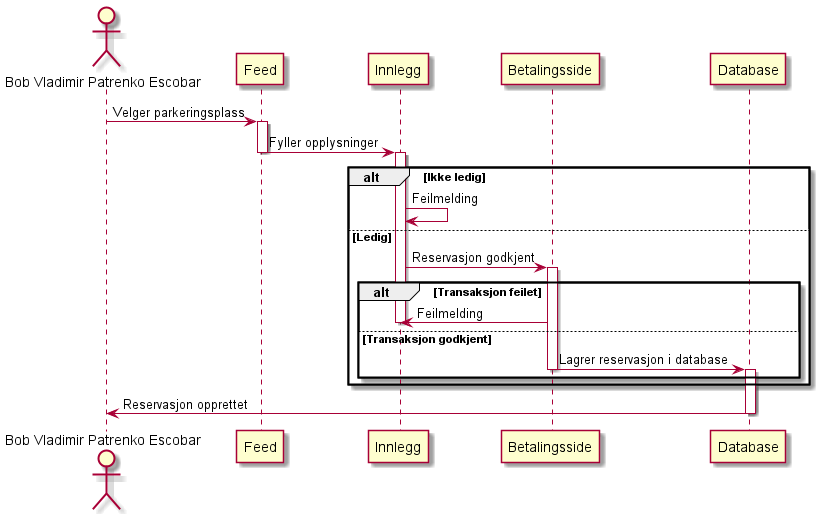
\includegraphics[max width=\textwidth]{bilder/diagrammer/opprette reservasjon_sekvensdiagram.png}

    \subsection{Tilstandsdiagram - Registrere parkeringsplass}
    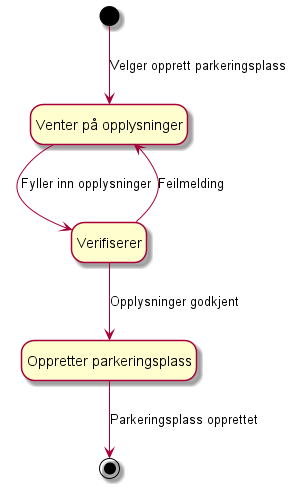
\includegraphics[max width=\textwidth]{bilder/diagrammer/opprett_parkeringsplass_tilstandsdiagram.png}
    
        \subsubsection{Forklaring}
        Når bruker oppretter parkeringsplass venter systemet på en POST forespørsel med informasjon om gatenavn, adresse, bredde, lengde og høyde, samt informasjon angående parkeringsplasstype (handicap, el-bil, osv.). Dersom opplysningene ikke tilfredstiller forventningene i systemet, får bruker en feilmelding og blir nødt til å fylle ut på nytt. Dersom opplysningene er godkjent blir parkeringsplassen opprettet. 

    \subsection{Aktivitetsdiagram - Leie en parkeringsplass}
    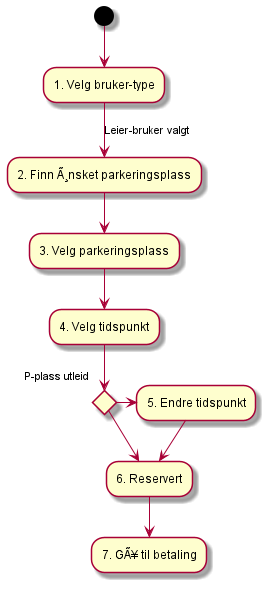
\includegraphics[max width=\textwidth]{bilder/diagrammer/leierAktivitetBestilling.png}

    \subsection{Sekvensdiagram - Leie ut en parkeringsplass}
    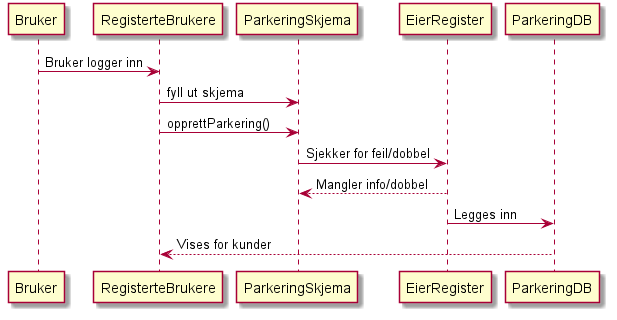
\includegraphics[max width=\textwidth]{bilder/diagrammer/sekvensdiagramLeggeUtParkering.png}

    \subsection{Dataflytdiagram - Opprett Parkeringsplass}
    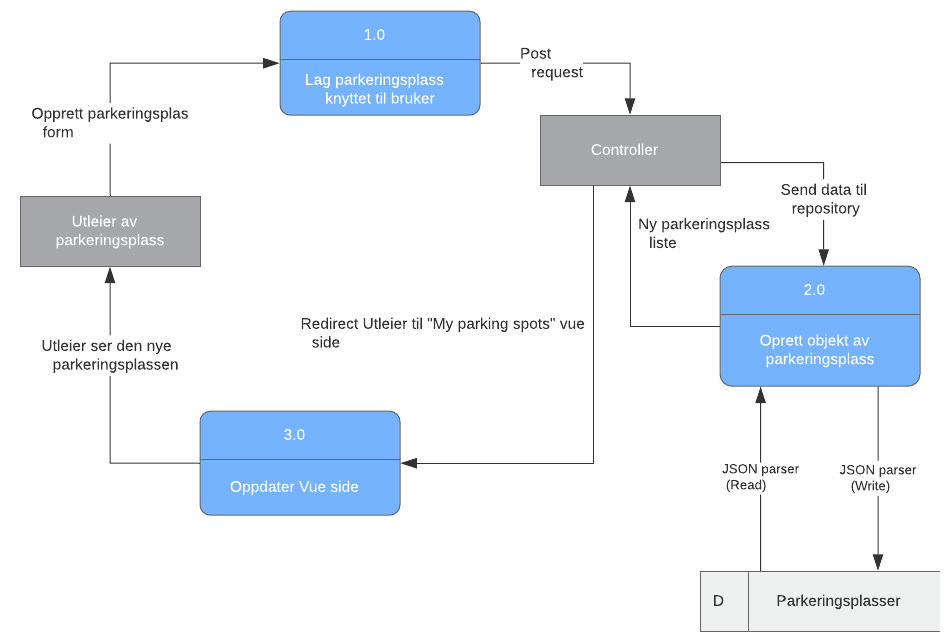
\includegraphics[max width=\textwidth]{bilder/diagrammer/DataflytOpprettParkering.png}

\section{Estemering}

    \subsection{Enheter}

    \begin{tabular}{|p{2cm}|
        >{\centering\arraybackslash}p{3cm}|
        >{\centering\arraybackslash}p{3cm}|
        >{\centering\arraybackslash}p{3cm}|
        >{\centering\arraybackslash}p{3cm}|}     
        \hline 
        \invis & \multicolumn{4}{|c|}{Utviklingsstørrelse}\\
        \hline
        Verdi & X-Large & Large & Medium & Small\\
        \hline
        X-Large &   \celly0 &
                    \cellg4 &
                    \cellg6 &
                    \cellg7 \\
        \hline
        Large &     \cellr-4 &
                    \celly0 &
                    \celll2 &
                    \cellg3 \\
        \hline
        Medium &    \cellr-6 &
                    \cello-2 &
                    \celly0 &
                    \celll1 \\
        \hline
        Small &     \cellr-7 &
                    \cellr-3 &
                    \cello-1 &
                    \celly0 \\
        \hline 
    \end{tabular}

    \subsection{Estimeringstabell - Funksjonelle krav}

    \begin{longtable}{|p{2cm}|p{6cm}|
        >{\centering\arraybackslash}p{2cm}|
        >{\centering\arraybackslash}p{2cm}|
        >{\centering\arraybackslash}p{2cm}|} 
        \hline
        \bf ID & \bf Krav & \bf Vikitighet & \bf Utviklingstid & \bf Størrelse\\
        \hline
        FK1
        &
        Bruker skal kunne opprette en brukerkonto
        & M & M & \celly 0\\
        \hline
        FK2
        &
        Bedrifter skal kunne opprette en bedriftskonto
        & M & M & \celly 0\\
        \hline
        FK3
        &
        Kunden skal kunne opprette brukerkonto med administratorrettigheter
        & S & M & \cello -1\\
        \hline
        FK4
        &
        Systemet skal verifisere registreringen
        & L & L & \celly 0\\
        \hline
        FK5
        &
        Dirigere opprettet bruker
        & S & S & \celly 0\\ % implementert
        \hline
        FK6
        &
        Bruker skal kunne logge inn som en brukerkonto eller bedriftskonto
        & XL & M & \cellg 6\\
        \hline
        FK7
        &
        Systemet skal verifisere innloggingen
        & XL & S & \cellg 7\\
        \hline
        FK8
        &
        Dirigere innlogget bruker
        & S & S & \celly 0\\
        \hline
        FK9
        &
        Systemet skal verifisere bruker gjennom en kode
        & XL & L & \cellg 4\\
        \hline
        FK10
        &
        Feeden skal oppliste relevante parkeringsplasser
        & XL & M & \cellg 6\\
        \hline
        FK11
        &
        Bruker skal kunne sette et filter på feeden
        & L & XL & \cellr -4\\
        \hline
        FK12
        &
        Bruker skal kunne søke etter en lokasjon
        & M & L & \cello -2\\
        \hline
        FK13
        &
        Bruker skal kunne leie parkeringsplass som en brukerkonto
        & XL & M & \cellg 6\\
        \hline
        FK14
        &
        Varsel på utløpstid
        & M & M & \celly 0\\
        \hline
        FK15
        &
        Bruker skal kunne gi tilbakemelding på et innlegg
        & S & L & \cellr -3\\
        \hline
        FK16
        &
        Tilbakemeldinger skal vises på hvert innlegg
        & S & M & \cello -1\\
        \hline
        FK17
        &
        Utleier skal kunne få tilbakemeldingene via e-post
        & S & S & \cellg 0\\
        \hline
        FK18
        &
        Brukerkonto og bedriftskonto skal kunne registrere en eller flere parkeringsplasser
        & XL & XL & \cellg 0\\
        \hline
        FK19
        &
        Pris per time skal bestemmes av utleier
        & M & S & \celll 1\\
        \hline
        FK20
        &
        Tiden skal bestemmes av bruker
        & L & M & \celll 2\\
        \hline
        FK21
        &
        Brukere skal kunne se ut ifra innlegget om parkeringsplassen er ledig eller ikke
        & L & M & \celll 2\\
        \hline
        FK22
        &
        Bruker skal betale utleieren for å opprette en reservasjon
        & L & M & \celll 2\\
        \hline
        FK23
        &
        Tredjepart
        & L & S & \cellg 3\\
        \hline
        FK24
        &
        Administrator skal kunne bannlyse bruker
        & S & S & \celly 0\\
        \hline
        FK25
        &
        Administrator skal kunne slette bruker
        & M & S & \celll 1\\
        \hline
        FK26
        &
        Administrator skal kunne slette tilbakemeldinger
        & S & S & \celly 0\\
        \hline
        FK27
        &
        Administrator skal kunne slette innlegg
        & L & S & \cellg 3\\
        \hline
        FK28
        &
        Administrator skal kunne slette parkeringsplasser
        & L & S & \cellg 3\\
        \hline
        FK29
        &
        Administrator skal kunne slette reservasjoner
        & XL & S & \cellg 7\\
        \hline
        FK30
        &
        Bedrift skal ha administrerende rettigheter på deres egne innlegg
        & S & M & \cello -1\\
        \hline
        FK31
        &
        Bruker skal kunne rapportere andre brukere sine innlegg
        & M & S & \celll 1\\
        \hline
        FK32
        &
        Bruker skal kunne rapportere andre brukere
        & M & S & \celll 1\\
        \hline
        FK33
        &
        Systemet skal lagre informasjon om parkeringsplasser
        & XL & XL & \celly 0\\
        \hline
    \end{longtable}

    \subsection{Estimeringstabell - Ikke funksjonelle krav}

    \begin{longtable}{|p{2cm}|p{6cm}|
        >{\centering\arraybackslash}p{2cm}|
        >{\centering\arraybackslash}p{2cm}|
        >{\centering\arraybackslash}p{2cm}|}
        \hline
        \bf ID & \bf Krav & \bf Vikitighet & \bf Utviklingstid & \bf Størrelse\\
        \hline
        IFK1
        &
        Tilgjengelighet
        & XL & XL & \celly 0\\
        \hline
        IFK2
        &
        Bruker kvalifikasjon
        & L & M & \celll 2\\
        \hline
        IFK3
        &
        Sikkerhetskopi(Backup)
        & XL & S & \cellg 7\\
        \hline
        IFK4
        &
        Dependency på tredjepart
        & XL & S & \cellg 7\\
        \hline
        IFK5
        &
        Legal and licensing issues
        & L & M & \celll 2\\
        \hline
        IFK6
        &
        Response time - Lokalt
        & S & L & \cellr -3\\
        \hline
        IFK7
        &
        Page loading
        & S & M & \cello -1\\
        \hline
        IFK8
        &
        Personvern
        & XL & XL & \celly 0\\
        \hline
        IFK9
        &
        Sikkerhet
        & XL & L & \cellg 4\\
        \hline
        IFK10
        &
        Supportability
        & M & L & \cello -2\\
        \hline
        IFK11
        &
        Usability
        & S & M & \cello -1\\
        \hline
        IFK12
        &
        Compliance
        & M & S & \celll 1\\
        \hline
    \end{longtable}

\end{document}